\documentclass[conference]{IEEEtran}

% --- IDIOMA ---
\usepackage[spanish, es-tabla]{babel}

% --- FUENTES (XeLaTeX) ---
\usepackage{fontspec}
\setmainfont{Liberation Serif}
\setmonofont{JetBrainsMono Nerd Font}

% --- CITAS IEEE ---
\usepackage[backend=biber,style=ieee,sorting=none]{biblatex}
\addbibresource{referencias.bib}

% --- UTILIDADES ---
\usepackage{graphicx}
\usepackage{float}
\usepackage{amsmath}
\usepackage{booktabs}
\usepackage[colorlinks=true,linkcolor=black,citecolor=black,urlcolor=blue]{hyperref}

% --- CÓDIGO ---
\usepackage{xcolor}
\definecolor{bg}{RGB}{40,44,52}

\usepackage{minted}

\setminted{
  style=monokai,
  bgcolor=bg,
  breaklines,
  breakanywhere=true,
  tabsize=2,
  fontsize=\footnotesize
}

\usepackage{csquotes}

\begin{document}



% --- INICIO DE LA PORTADA ---
\begin{titlepage}
    \centering
    \vspace*{0.5cm}
    
    % --- Escudo de la UV ---
    % Asegúrese de tener el archivo "escudo_uv.png" (o .jpg) en su carpeta del proyecto
    
\includegraphics[width=0.3\textwidth]{UV.png} \\ 
    \vspace{0.8cm}
    
    {\huge \textbf{Universidad Veracruzana}} \\
    \vspace{0.4cm}
    {\Large Facultad de Instrumentación Electrónica} \\ % Corregido: Instrumentación
    \vspace{0.2cm}
    {\large Ingeniería Biomédica} \\
    
    \vfill
    
    % Título de la Experiencia Educativa y Actividad
    {\Large \textbf{EE: Interfaces Hombre-Máquina}} \\
    \vspace{0.8cm}
    {\Large \textbf{ACTIVIDAD 03. JOYSTICK COMO DISPOSITIVO PARA UNA INTERFAZ HOMBRE-MÁQUINA}} \\
    
    \vspace{1.5cm}
 
    % Información de los Integrantes
    \begin{flushright} % Alineado a la derecha para un toque más profesional
        \textbf{Profesor:} \\
        Varela Lara Luis Julian \\
        \vspace{0.5cm}
        \textbf{Integrantes del equipo ``\textit{ES3.14}}'': \\
        Alfonso Gamboa Rubén \\
        Flores Montero Edsel Yetlanezi \\
    \end{flushright}
    
    \vfill
    
    {\large \textbf{Fecha:} 8 de abril de 2026} \\
    \vspace{1cm}
    {\small Xalapa, Enríquez, Ver.} % O la sede correspondiente
\end{titlepage}
% --- FIN DE LA PORTADA ---



% --- EL CUERPO DEL TEXTO (Automáticamente en dos columnas) ---

\section{Introducción al tema.}
El siguiente reporte incluye la información empleada para la construcción, explica la lógica del control y la integración de los dispositivos HW-504 y Arduino con el objetivo de establecer un sistema físico (Hardware) qué permita interactuar en tiempo real con el programa ``ComandosRS232''.

\section{Marco teórico.}
  \subsection{ARDUINO.}
    \subsubsection{Conversión Analógico-Digital (ADC)}
    Los microcontroladores de la familia Arduino cuentan con conversores ADC de 10 bits. Es decir, pueden leer variaciones de voltaje de 0V a 5V y traducirlas en un rango de valores enteros que va de 0 a 1023. En un estado de reposo ideal, el joystick arrojará un valor aproximado a 512 en ambos ejes.
    \subsubsection{Comunicación}
    RS232 (Serial): Es un estándar de comunicación asíncrona. Permite el intercambio de datos entre el microcontrolador y la computadora. A través del puerto USB (Emulando COM).

    \subsubsection{Modulo Joystick HW-504}
    El HW-504 es un periférico analógico-digital enfocado en la interacción de interfaces hombre-máquina (HMI) con microcontroladores. Está compuesto por dos potenciómetros acoplados a un mecanismo de cardán (sistema mecánico que permite transmitir movimiento de rotación entre dos ejes no alineados), para los ejes X e Y y un botón (para el eje Z). Las dimensiones aproximadas del periférico son 34 mm x 26 mm x 32 mm.

    \subsubsection{Funcionamiento}
    El voltaje de operación compatible con lógica de 3.3V y 5V DC. Internamente funciona mediante dos potenciómetros de 10 kΩ dispuestos perpendicularmente para detectar el movimiento a lo largo de los ejes X e Y, junto con un botón que se activa al presionar la palanca del joystick.

    En una posición central, el potenciómetro se encuentra completamente equilibrado, por lo qué al actual como un divisor de voltaje entrega un voltaje de salida igual a cada una de las salidas.

    Al mover la palanca, la resistencia del potenciómetro funciona como un divisor de voltaje qué permite incrementar el voltaje de salida con preferencia hacia una de las salidas dependiendo de la dirección y movimiento de la palanca.

    La salida digital del módulo (pin SW) funciona como un interruptor normalmente abierto que se conecta a tierra cuando se pulsa, lo que da lugar a una señal LOW; permanece abierto (lectura HIGH con una resistencia pull-up) cuando se suelta.

    \subsubsection{Pines (conexión)}
    \begin{itemize}
      \item GND (Ground): Tierra
      \item +5V (o VCC): DC (5-3.3V)
      \item VRx (Voltaje Referencia X): Salida analógica del eje horizontal. Pin analógico (A0).
      \item VRy (Voltaje Referencia Y): Salida analógica del eje vertical. Pin analógico (A1).
      \item SW (Switch): Botón digital. Activar una resistencia pull-up. 
        \begin{itemize}
          \item Sin pulsar, leerá un valor ALTO (1),
         \item Presionado, leerá un valor BAJO (0).
        \end{itemize}
    \end{itemize}

  \subsection{Diseño del sistema.}
    \subsubsection{Interconexión HW-504 - Arduino}
    \begin{itemize}
      \item GND (Ground) HW-504 - GND (Ground) Arduino
      \item +5V (o VCC) HW-504 - +5V Arduino
      \item VRx (Voltaje Referencia X) - Pin Analógico A0 Arduino
      \item VRy (Voltaje Referencia Y) - Pin analógico A1 Arduino
      \item SW (Switch) - Pin Digital 2 Arduino (Activar:INPUT\_PULLUP)
    \end{itemize}

    \subsection{Diseño del Control}
    En esta sección se explica la información necesaria empleada para diseñar la interfaz Hombre-Maquina (HMI), la lógica empleada para convertir el voltaje analógico a voltaje digital y su posterior incorporación en el código diseñado para controlar el programa ComandosRS232.

    \subsubsection{Zonas Muertas (Deadzone)}
    Debido a las características mecánicas de los potenciómetros, las lecturas analógicas del periférico pueden no regresar el mismo punto central debido a las tolerancias físicas de los potenciómetros, por lo qué es necesario considerar una zona en la qué el valor será considerado el mismo valor del punto central. A esté espacio se le denominará como “Velocidad Cero” o “Punto muerto”/”DeadZone”.

    Para la calibración ideal del eje, se establece en la posición 496 para el eje X y 524 para el eje Y. Definió qué el margen de tolerancia para esté punto muerto tendrá una tolerancia de 0.02 (2%). Es decir qué mientras la palanca se posicione a una distancia (496, 524)+-2% el valor de la lectura será igual a (496, 524)

    Cualquier posición (otorgada por la lectura actual) fuera de esté rango, asignará un un valor igual a 1 (incremento) y/o -1 (decremento) en su vector correspondiente. Dentro del rango del punto muerto, el valor de dirección será igual a 0.

    \subsubsection{Velocidad de Desplazamiento}
    Tanto para la sección "CAMBIA VALOR" (que requiere cuatro velocidades: cero, baja, media y alta) como para "RECORTAR IMAGEN" (tres velocidades). Para tener un perfil de aceleración qué nos permite un rango de movimientos precisos en la zona central y rapidez extrema en los extremos, se empleó un algoritmo cuyo comportamiento simula una curva de aceleración exponencial.

    Esta sensibilidad exponencial nos permitirá navegar rápidamente (extremos) por la imagen y luego ralentizar el cursor (área central) para colocar con precisión en las posiciones deseadas 

    
La posición del joystick es convertida en una frecuencia de transmisión de acuerdo con la siguiente función matemática:
$$f(p) = |511 - p^a| \cdot \frac{f_{max}}{511^a} $$

Donde:
\begin{itemize}
  \item $f(p)$ es la frecuencia resultante en hercios (Hz).
  \item $p$ es la lectura analógica actual.
  \item $a$ es el factor de aceleración.
    \begin{itemize}
      \item Un valor menor resultará en una curva más aplanada (aceleración más baja  en la zona exterior)
      \item Un valor mayor resultará en una curva más cerrada (aceleración más alta en la zona exterior)
    \end{itemize}
  \item $f_{max}$ es la frecuencia máxima permitida.
 \begin{itemize}
      \item Un valor menor resultará en una curva más ``corta'' (aceleración más alta en la zona interior)
      \item Un valor mayor resultará en una curva más ``amplia'' (aceleración más baja en la zona interior)
    \end{itemize}
  \end{itemize}

  Tanto los  valores a / fmax, pueden ser modificados directamente desde el código de la placa del microcontrolador. 

    \subsubsection{Movimiento diagonal (asincronia)}
    Dado que el joystick puede permitir movimientos en diagonal, los ejes X e Y deben procesarse simultáneamente. Dado qué el valor anterior fue calculado en el dominio de la frecuencia, es necesario qué esté valor sea transformado ha milisegundos, para permitir qué el reloj interno del microcontrolador pueda evaluar correctamente la información.
    $$milis(T) = \frac{1000}{f(p)}$$
    Esto permite qué los valores de los ejes X e Y puedan ser transmitidos en hilos independientes evitando la interferencia mutua. Se evitó el uso de (delay())  ya qué esté bloquea el funcionamiento del microcontrolador.

    \subsubsection{Botón del joystick}
    El pulsador del joystick (SW) se utiliza para indicar los puntos dónde iniciará el área de corte. Se configuró el pin digital con resistencia interna (INPUT\_PULLUP), lo que invierte su lógica (estado de reposo ALTO, presionado BAJO).

    El Arduino solo transmite el comando maestro 50 vía RS232 en el instante exacto en que detecta la transición de BAJO a ALTO (cuando se suelta el botón).


\section{Dearrollo de la actividad.}
  \subsection{Desarrollo del código.}
  La estructura usada para el el código es:
  \begin{enumerate}
    \item \textbf{Declaració de variables y constantes.} Se hacen al inicio para que el arduino sepa como interpretarlas una vez inicie el programa, sin tener que declararlas cada ciclo del loop, esto reduce lentitudes en el programa. Además, tener bien ubicadas a las variables y constantes permite tambien usarlas como un pseudo menú de configuración o de ajustes.
    \item \textbf{Definición de funciones.} Aunque en Arduino no afecte mucho el donde se declaren las funciones que se van a usar, es buena práctica declararlas desde el principio, permitiendo comprensión más sencilla del código, esto facilitando la resolución de errores a largo plazo.
    \item \textbf{setup().} Corresponde a lo que hace el microcontrolador una sola vez que arranca.
    \item \textbf{loop().} Dentro de este bloque de código, el microcontrolador va a repetir las instrucciones infinitamente.
  \end{enumerate}

  \paragraph{Variables y Constantes}
  \begin{enumerate}
    \item \textbf{Pines.} Declarar los pines al principio permite que sea sencillo tanto consultar como sebería ser la conección, pues el error más común es un mal armado de circuito. Además el que estén en variables, permite que si en un futuro hay que cambiar algún pin, este cambio se apique de forma sencilla. El Joystick tiene 2 pines analógicos: Vx y Vy que corresponden respectivamente a las coordenadas de donde se encuentra la palanca, por eso les asignamos los pines analógicos A1 y A2 del arduino; también cuenta con un pin digital: SW, el cual va a estar conectado al pin digital 7 del arduino.
    \item \textbf{Variables de tiempo.} Nos van a permitir guardar el tiempo, por lo que se usa \textit{long} para guardar grandes cantidades de bits(pues vamos a guardar milisegundos) y \textit{unsigned} para indicar que no usaremos números negativos, al no usar numeros negativos, podemos almacenar números enteros más grandes todavía. tiempoAnteriorX y tiempoAnteriorY nos permitirán guardar el tiempo del ultimo cambio que han tenido X y Y respectivamente, por lo que les asignamos un valor default de 0.
    \item \textbf{Periodos y frecuencias. }Estas variables serán utilizadas en conjunto con una función que nos va a permitir jugar con la frecuencia y el periodo de impresión de números en el puerto serial.
    \item \textbf{Varialbles de estado. } Estas variables harán juego con una segunda función que se declarará más adelante, la cual nos dará la dirección de hacia donde está el Joystick. Como no queremos que el boton inicie en \textit{true}, le asignamos un valor default de \textit{false}.
    \item \textbf{Constantes del Joystick. } Estas constantes nos van a permitir guardar \textit{El valor que tienen las coordenadas X y Y del Joystick cuando la palanca se encuentra en medio}, pues queremos saber \textit{dónde está el Joystick cuando está en el centro.} Estos valores se obtuvieron de registrar la posición del Joystick, siendo 496 el centro del eje X y 524 el centro el eje Y.
    \item \textbf{Configuración.} Guardamos como constantes: la velocidad máxima en Hz que tendrá de impresión cuando el Joystick se encuentre en el tope,  el nivel de asceleración (2 equivale a una asceleración cuadrada), y la toleracia con respecto al centro,  pues el Joystick aún estando en el centro, sus valores llegan a variar ligeramente.
  \end{enumerate}
  
  \paragraph{Funciones}
  Para el desarrollo de esta actividad solo se definieron dos funciones, una que permite convertir la distancia del joystick del centro en una frecuencia (figura \ref{fig:funcion}) y otra que permite conocer hacia que dirección está apuntando el Joystick.
  \begin{figure}[h]
      \centering
      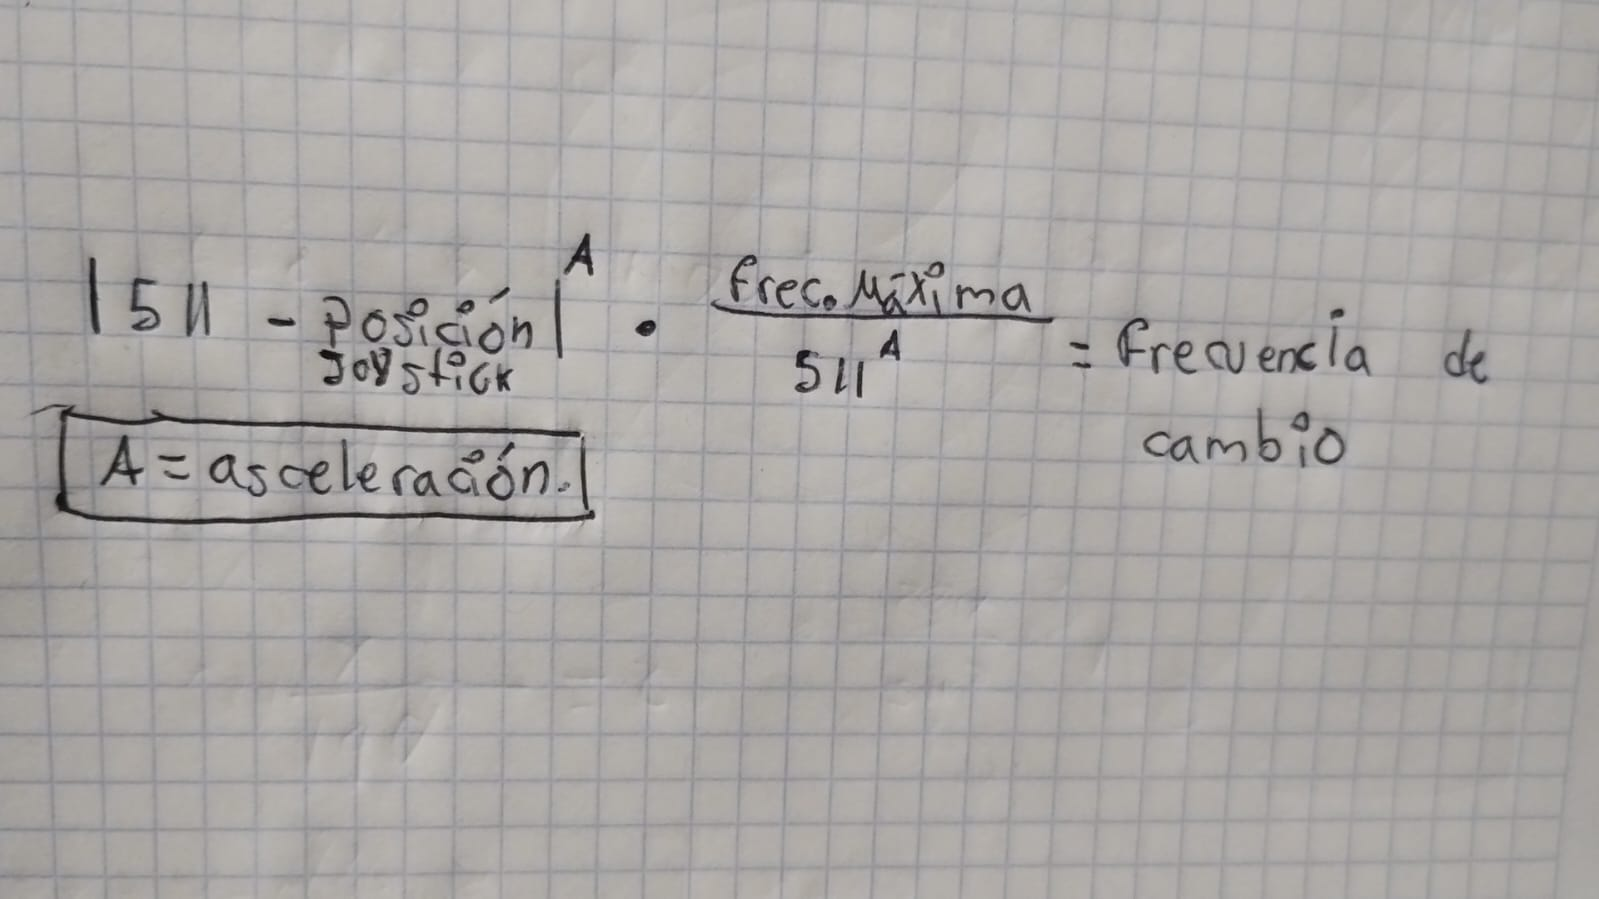
\includegraphics[width=\linewidth]{Funcion1.jpg} % \linewidth se ajusta a la columna
      \caption{Ilustración matemática de como funciona esta función 1}
      \label{fig:funcion}
    \end{figure}
  
    \paragraph{setup()}
    Para esta seccion simplemente se inicia la comunicación serial de 9600 baudios y se inician los pines como INPUT (INPUT\_PULLUP para el botón).

    \paragraph{loop()}
    Dentro del loop ya podemos leer en cada instante los valores que toman X y Y,  mientras almacenamos el tiempo actual.
    Para la siguiente parte del loop a travez de ifs detectamos si ha transcurrido un tiempo mayor al periodo preestablecido anteriormente, e imprimimos, pudiendo así respetar la velociadad sin usar delays. 
    $$ if (\Delta tiempo\_transcurrido >= periodo\_cambio) \{$$
    $$ sube\_o\_baja$$
  $$\}$$
    
    repitiendo este códiga tanto para X como para Y.
    
    Finalmente para el botón solo se añade una verificación de pulso.


  \begin{figure}[t]
      \centering
      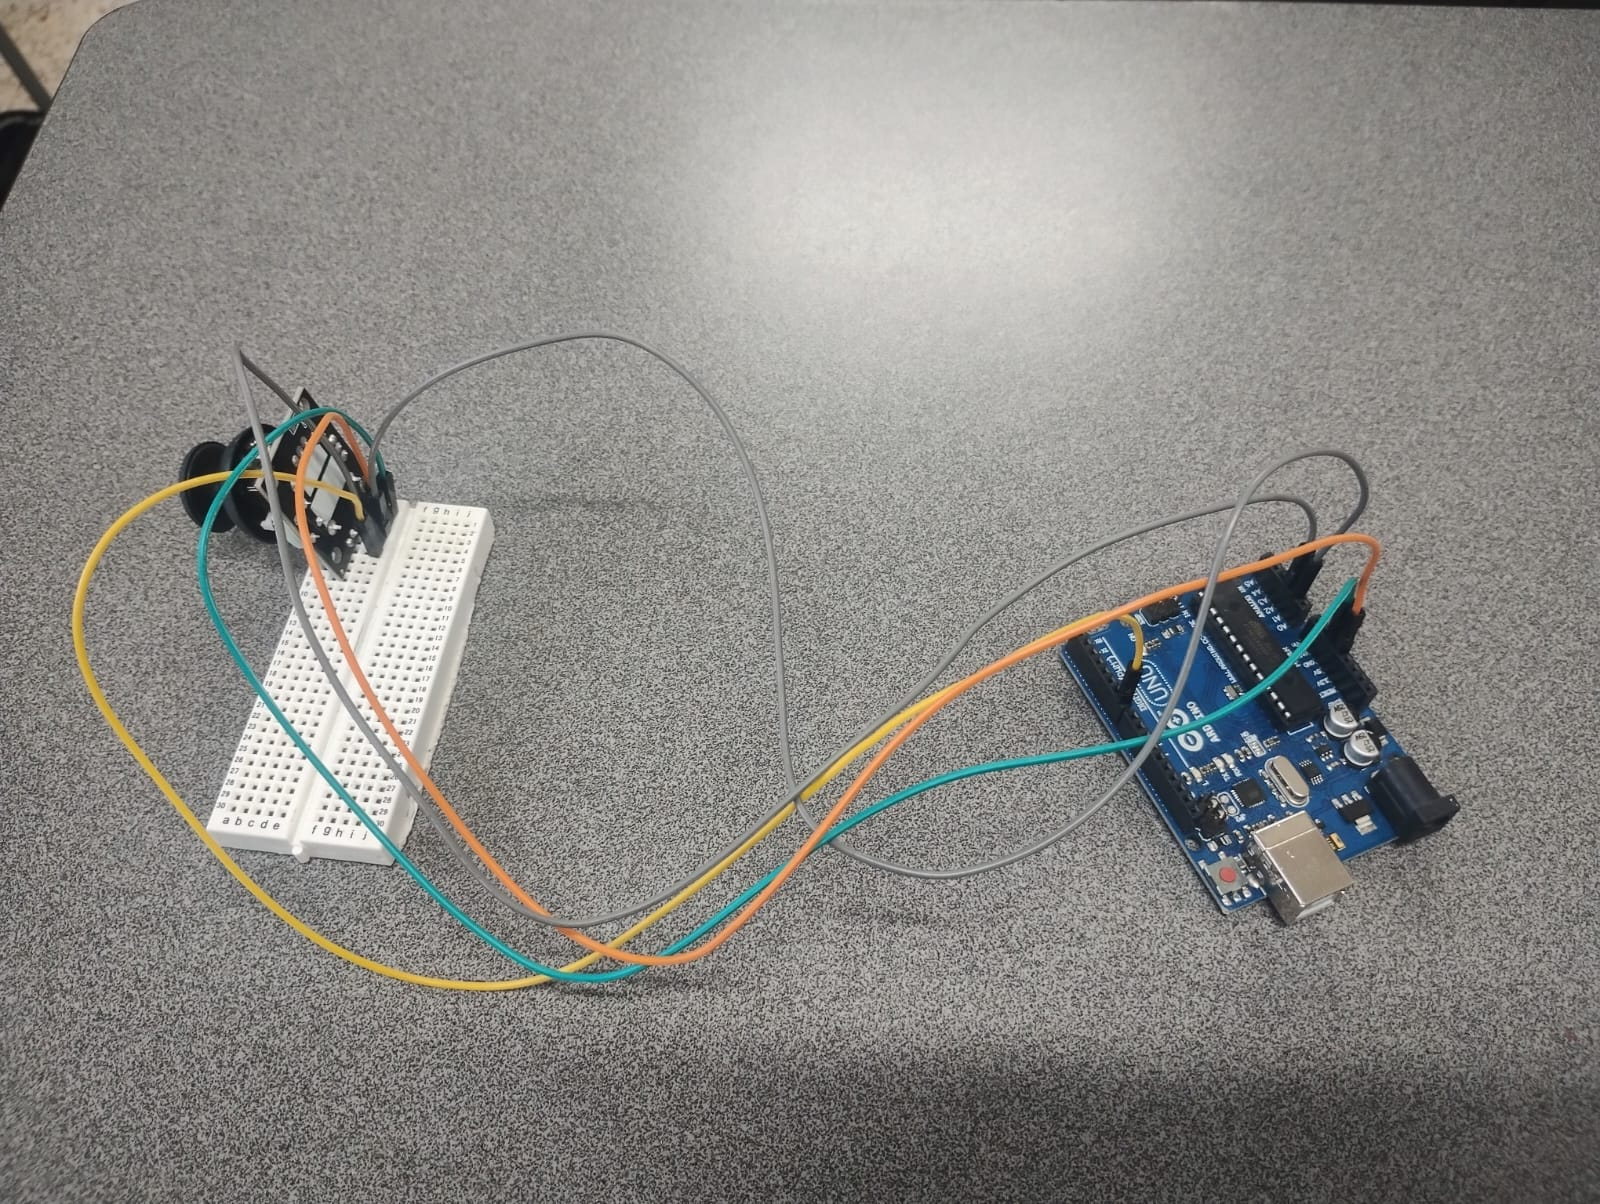
\includegraphics[width=\linewidth]{circuito.jpg} % \linewidth se ajusta a la columna
      \caption{circuito armado}
      \label{fig:circuito}
    \end{figure}

  \newpage
  \subsection{Código completo}
    A continuación se deja el código completo usado durante el desarrollo de esta actividad:
    \inputminted{cpp}{Act03.ino}



\section{Conclusiones}
El desarrollo de esté proyecto nos ejemplifica como la inclusión de componentes básicos como un un potenciómetro y conceptos eléctricos como el divisor de voltaje pueden ser utilizados para formar sistemas más completos con un perfil de movimiento más amplio. Ya qué tipo de componente se pueden adquirir fácilmente en cualquier tienda de electrónica, incrementa las opciones y funciones disponibles para incorporar en otros proyectos enfocados en Interfaces Hombre-Máquina qué puedan requerir esté tipo de manipulación. La incorporación de un microcontrolador nos ofrece una enorme cantidad de opciones para integrar esté dispositivo físico en cualquier tipo de software. Sin embargo, el conocimiento de programación, electrónica, y matemáticas, entre los qué puedo nombrar en esté momento, nos ofrecen un gran abanico de oportunidades para poder mejorar notablemente la calidad de la respuesta en el software, como en esté caso la incorporación de conceptos matemáticos nos brindó una herramienta qué simplifica un proceso de diseño, y teóricamente la incorporación de sistemas electrónicos anti bounces benefician la precisión del movimiento al poder reducir o eliminar por completo las oscilaciones analógicas que se ven reflejadas como movimiento indeseado en el software.

\newpage{}
\section{firma de revisión}
\begin{figure}[h]
    \centering
    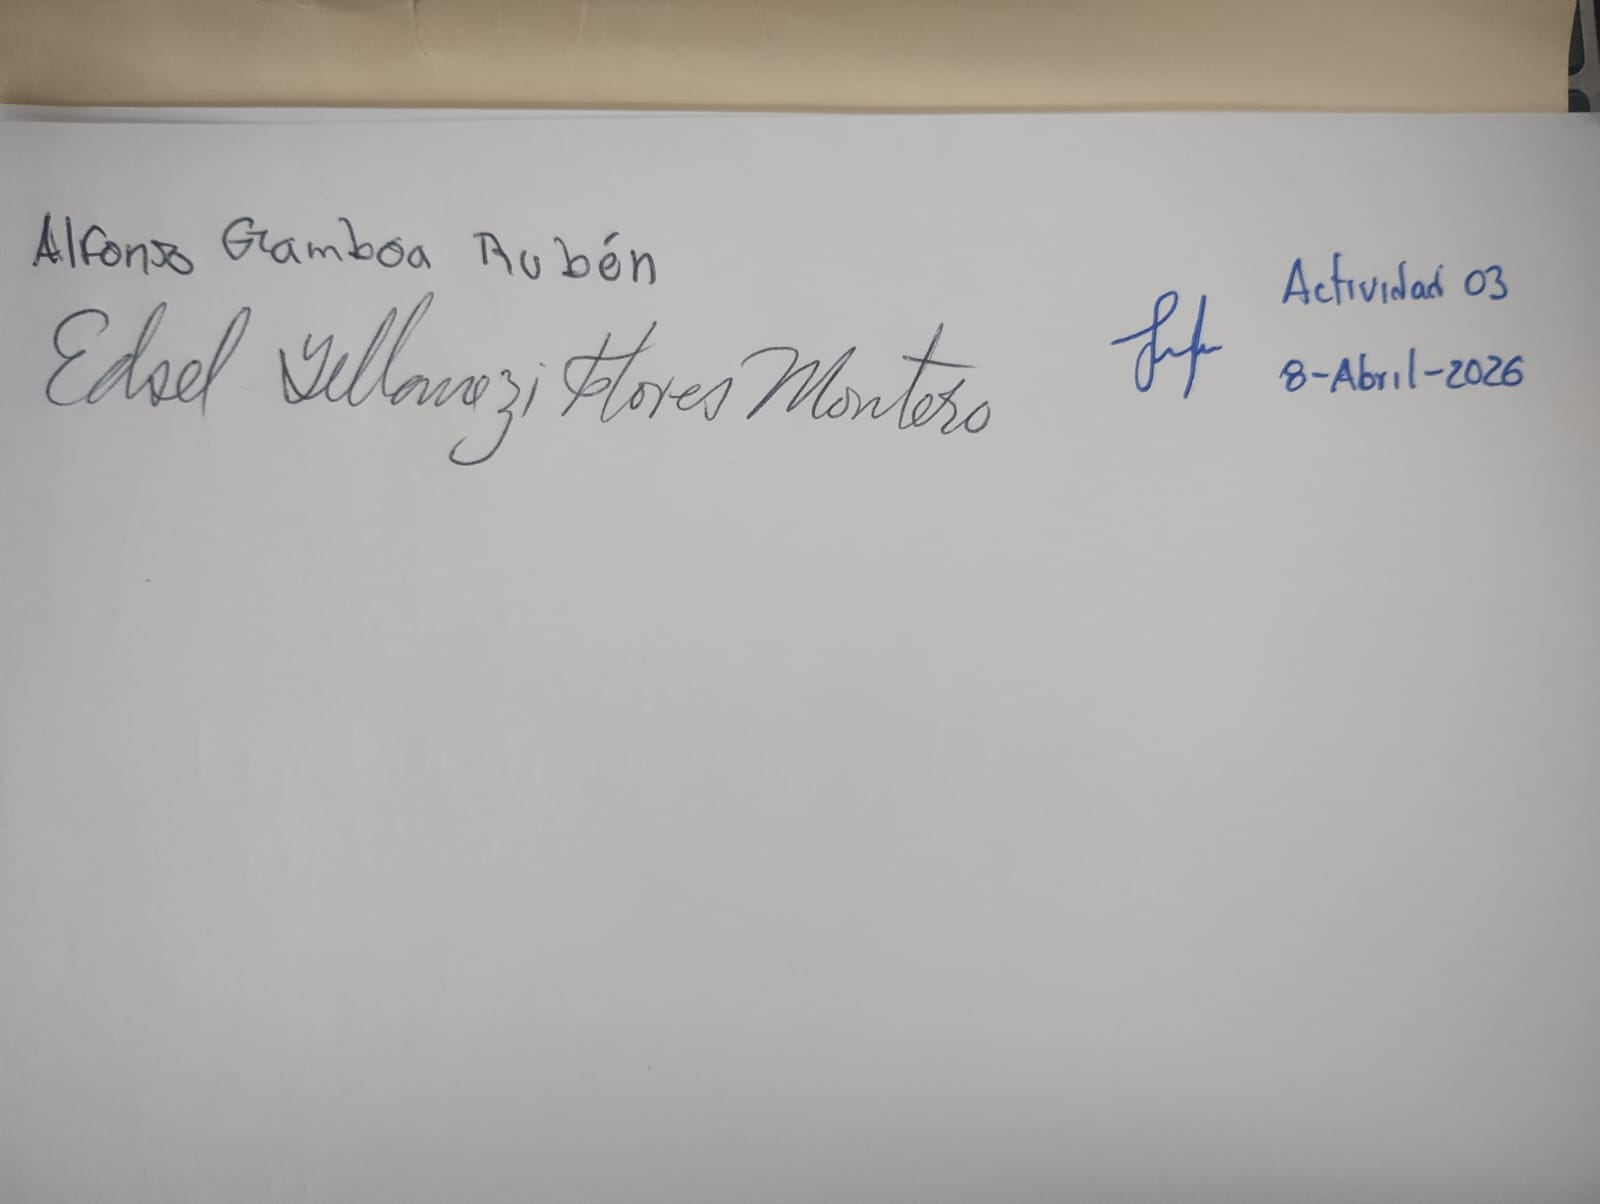
\includegraphics[width=\linewidth]{Firma.jpg} % \linewidth se ajusta a la columna
    \caption{Firma de revisión}
    \label{fig:Firma}
\end{figure}



% --- REFERENCIAS ---
%\printbibliography

\begin{thebibliography}{9}

\bibitem{arduino_2023}
Arduino LLC. (2023). \textit{analogRead() - Arduino Reference}. Recuperado de https://www.arduino.cc/reference/en/language/functions/analog-io/analogread/

\bibitem{axelson_2007}
Axelson, J. (2007). \textit{Serial Port Complete: COM Ports, USB Virtual COM Ports, and Ports for Embedded Systems} (2da ed.). Lakeview Research LLC.

\bibitem{llamas_2016}
Llamas, L. (2016). \textit{Leer un Joystick analógico con Arduino}. Luis Llamas: Ingeniería y Maker. Recuperado de https://www.luisllamas.es/leer-un-joystick-analogico-con-arduino/

\bibitem{prometec_2015}
Prometec. (2015). \textit{El Joystick y los pines analógicos}. Prometec.net. Recuperado de https://www.prometec.net/joystick/

\bibitem{tocci_2007}
Tocci, R. J., Widmer, N. S., \& Moss, G. L. (2007). \textit{Sistemas digitales: principios y aplicaciones} (10ma ed.). Pearson Educación.

\end{thebibliography}

\end{document}
